% \newcommand\ceil[1]{\lceil {#1} \rceil}
% \newcommand\floor[1]{\lfloor {#1} \rfloor}

\newcommand\scalarprod{\cdot}
\newcommand\oequal{~\oplus \hspace{-0.3em} =}
\newcommand\rank{\textrm{rank}}
\newcommand\hweight{\textrm{hw}}
\newcommand\field[1]{\mathbb{F}_{2}^{#1}}
\newcommand\gf[1]{\mathbb{F}_{2^{#1}}}
\newcommand\anf{\mathsf{anf}}
\newcommand\anfAbbrev{ANF}
\newcommand\rmax[2]{r_{\textrm{max}}(#1, #2)}
\newcommand\kroenecker[2]{[#1 = #2]}
\newcommand\indicator[1]{\mathbb{I}_{#1}}

\newcommand\cstyle[2]{#1 = (\mathtt{#2})}

\newcommand\smallcite[1]{{\color{gray}\footnotesize\cite{#1}}}

\newcommand\etal{{\it et al.}}

\newcommand\HEIGHT{}
\newcommand\FigTex[2]{
\renewcommand\HEIGHT{#1}
\input{figures/#2}
}

\setcounter{MaxMatrixCols}{20} % increase matrix size

\newcommand{\TITLE}{}

\newcommand\Title[1]{
\begin{center}
    \Large #1
\end{center}
}

\newcommand\CurTitle{\Title{\TITLE}}

\newcommand\Center[1]{\begin{center}#1\end{center}}
\newcommand\CenterBlock[2]{
\begin{center}
\begin{minipage}{#1}
#2
\end{minipage}
\end{center}}
\newcommand\Block[3]{\begin{textblock*}{#2}(#1)
#3
\end{textblock*}}

\newcommand\Grid{
\usebackgroundtemplate{
    \begin{tikzpicture}[remember picture,overlay]
        \draw[step=1cm,gray!20!white,thin,dashed] (current page.north west) grid (current page.south east);
        % \draw[step=1cm,gray!20!white,thin,dashed] (current page.south east) grid (current page.north west);
        \draw[ystep=3cm,xstep=4cm,gray!20!white,thin] (current page.south east) grid (current page.north west);
    \end{tikzpicture}
}
}


\newcommand\Footnote[1]{
\Block{0.5cm,8.5cm}{15.5cm}{
    \small \textcolor{Periwinkle}{#1}
}}
\newcommand\Credits[1]{
\Block{0.5cm,8.5cm}{8cm}{
    \small \textcolor{Periwinkle}{Figure credits: #1}
}}
\newcommand\CreditsTikz{
\Credits{\href{https://www.iacr.org/authors/tikz/}{TikZ for Cryptographers}}
}